\section{Personaggi}

\myframe{Cafer Paşa}{frame:cafer}{
  \setfarsi
  \novocalize
  \only<1>{
    \begin{center}
      \begin{tabular}{l@{\hspace{2cm}}r}
        \multicolumn{2}{c}{\includegraphics[scale=0.15]{parole/cafer.png}}\\
        Cafer, Mîr-i  mîrler-i Kıbrıs  & \RL{^g`fr mIri  mIrlar qubris}\\[1cm]
        \multicolumn{2}{c}{\footnotesize Cafer Paşa,  governatore di Cipro (vari mandati  dal 1003/1595).}\\[2mm]
        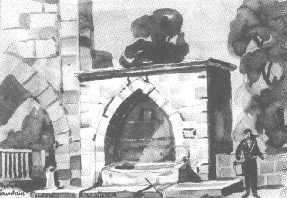
\includegraphics[scale=0.3]{atlas/cafer-fontana.png}
        &  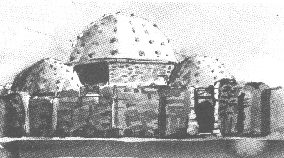
\includegraphics[scale=0.3]{atlas/cafer-bagno.png} \\
        1597 
        & 1601 \\
      \end{tabular}
    \end{center}
  }
  \only<2>{
    \begin{center}
      \begin{tabular}{p{0.48\textwidth}p{0.48\textwidth}}
        {\centering\includegraphics[scale=0.3]{documenti/vecellio295.png}}&
        {\centering\includegraphics[scale=0.4]{ritratti/Nadiri_f_8_v.jpg}}\\ 
        
        {\centering\tiny {\sc Cesare Vecellio}, {\it Habiti antichi et moderni
            di tutto il mondo}, Venezia, 1598}
        
        & {\centering\tiny
            {\it  Musicisti di fronte  a Mehmed  III}, Topkapı  Sarayı Müzesi,
            inv.  H889, f.  8, XVII  sec.} \\
      \end{tabular}
    \end{center}
  }

  \only<3>{
    \begin{center}
      \begin{tabular}{cc}
        \includegraphics[scale=0.25]{foto/aleppo-room-pergamon-1.png} &
        \includegraphics[scale=0.25]{foto/aleppo-room-pergamon-2.png} \\[1cm]
        \multicolumn{2}{c}{\tiny {\it Sala di Aleppo}, 1600-01, 
          Museums für Islamische Kunst (Pergamon), Berlin}\\ 
      \end{tabular}
    \end{center}
  }

}
